\documentclass[10pt,twocolumn,letterpaper]{article}

\usepackage{cvpr}
\usepackage{times}
\usepackage{epsfig}
\usepackage{graphicx}
\usepackage{amsmath}
\usepackage{amssymb}

% Include other packages here, before hyperref.

% If you comment hyperref and then uncomment it, you should delete
% egpaper.aux before re-running latex.  (Or just hit 'q' on the first latex
% run, let it finish, and you should be clear).
\usepackage[breaklinks=true,bookmarks=false]{hyperref}

\cvprfinalcopy % *** Uncomment this line for the final submission

\def\cvprPaperID{****} % *** Enter the CVPR Paper ID here
\def\httilde{\mbox{\tt\raisebox{-.5ex}{\symbol{126}}}}

% Pages are numbered in submission mode, and unnumbered in camera-ready
%\ifcvprfinal\pagestyle{empty}\fi
\begin{document}

%%%%%%%%% TITLE
\title{ClInKS: Classification of Individual KeyStrokes with Smartwatches}

\author{Anuj Kumar\\
College of Information and Computer Sciences\\
University of Massachusetts Amherst\\
{\tt\small anujkumar@umass.edu}
% For a paper whose authors are all at the same institution,
% omit the following lines up until the closing ``}''.
% Additional authors and addresses can be added with ``\and'',
% just like the second author.
% To save space, use either the email address or home page, not both
% \and
% Second Author\\
% Institution2\\
% First line of institution2 address\\
% {\tt\small secondauthor@i2.org}
}

\maketitle
%\thispagestyle{empty}

%%%%%%%%% ABSTRACT
\begin{abstract}
  Wearable consumer electronics with a myriad of sensors are becoming increasingly popular. With the boost in the popularity of smartwatches, the expectations from these devices are also on the rise. People desire more features than only counting steps. This project is aimed at a novel such use of a smartwatch-like device: to detect keystrokes typed on a classic QWERTY keyboard. Each key that one types is associated with a characteristic hand motion and frequency. Using time-series data provided by sensors inside the smartwatches worn on each hand of a user, we recover what is being typed on the keyboard. Since the data is affected only by the motion of one's hands, we show that a deep network learns to model these hand motions correctly. We hope to be able to recover the intended words typed by a user imitating typing on a keyboard in places where a physical keyboard is not readily available, thus reducing the reliance on a physical keyboard in one's daily life.
\end{abstract}

%%%%%%%%% BODY TEXT
\section{Introduction}
In the era of ubiquitous computing, it is becoming increasingly popular to rely on smart devices to improve our standard of living. The consumer electronics market has seen a steady rise in recent years in devices that carry several types of sensors. Smartwatches currently are undergoing the same boost in popularity that smartphones underwent about a decade ago.Since they are worn by individuals almost throughout the day, they offer a plethora of sensors to research. With an increasing number of users opting for these devices, the expectations on the capabilities of these devices also increases. They are now not just used for telling time and counting steps, but also for a number of daily tasks that is expected of smartphones. Most of the smartphone apps are being packaged for accompanying smartwatches for the sole purpose of making them readily accessible and easy to use.

Extending this thought, it's not uncommon for an app to require something for the user to type. Indeed, smartwatches have seen many novel ideas recently to enable typing. A few of those include typing on a QWERTY keypad on a very small screen as well as talking into the smartwatch and employing Natural Language Processing to convert it to text. These methods are cumbersome and might not be possible at all times. An individual is not in a noise-free zone or has the time and resources to concentrate on a tiny screen during an average part of their day.

As part of the Neural Networks course, this project aims at making the jump of rendering typing ubiquitous using only smartwatches. Being able to type on any surface regardless of background noise or context would make possible a lot more applications to be used in smartwatches. Consider the simple Facebook Messenger app\cite{messenger}. Currently the only corresponding function supported by a Messenger smartwatch extension is to open it on one's smartphone. We wish to be able to respond to anyone in real time, and if we had access to virtually a keyboard right 'on' our hands, applications like those could become more servicable.

Traditional work in the field of smartwatches has been restricted to using regression-based thresholds and then defining these thresholds for various activities. More recently, Machine Learning techniques have been used for classifying the time series data we get from sensors, by deriving statistical features from them, and then directly feeding it to a classifier. However, these methods are limited in their accuracy.

In this work, we obtain 9-axes real-life sensor data from each smartwatch worn on both hands while the user is typing normally. The data preprocessing step involves taking the time-series data around a typed character or word, and then assessing it in time as well as frequency space. This hand-built model of statistical features is then passed into a fully connected neural network for feature extraction. The output of this network is then passed into a recurrent neural network for the purposes of classification and prediction, and the complete network is trained end-to-end.

We show in this work, that the model is able to predict words typed by a user to mildly decent accuracy, even if the words don't belong to the English language. This is because the recurrent network learns the context of the letters in the background of other letters and can adapt to a particular person's specific typing slang. As a proof of concept, we show that given a smaller amount of words, the recurrent network easily fits the data and can predict every word correctly from the feature space provided to it. It would be interesting to see if the same model can be scaled to handle data coming from multiple people. This work has been left for future exploration.

This project is open-sourced and is available at \url{https://github.com/anujkumar93/DetectKeystroke}.
\begin{figure}[t]
\begin{center}
   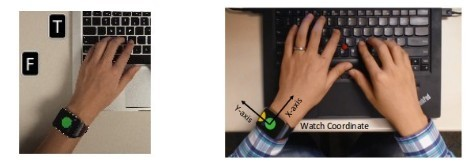
\includegraphics[width=0.99\linewidth]{./sample_image.jpg}
\end{center}
   \caption{Each typed character has a characteristic hand motion attached. The smartwatch can pick up on this characteristic motion.\cite{wang}\cite{maiti}}
\label{fig:sample}
\end{figure}

\section{Related Work}
Inferring meaningful activities from accelerometer data is not new. Early attempts involved a custom-made device to be worn at the hip for the explicit purpose of research. Ravi, et al. (2005)\cite{ravi} and Bonomi, et al. (2009)\cite{bonomi} used these custom-made devices to collect the data, extracted statistical features like mean, standard deviation, and cross-correlation, and then employed classification methods like decision trees and SVMs, and reported predictive performance in the ranges of 60\% to 99\% depending on the activity and setting.

With the advent of modern smartphones with accelerometers, studies made use of them as they were easily available and, more importantly, present in pockets of an ever-increasing number of people around the world. Kwapisz, et al. (2010)\cite{weiss} conducted studies in line with the works of \cite{ravi} and \cite{bonomi}, but for data collected using smartphones. They too relied on statistical features for classification - which involved multilayer perceptron and logistic regression among other techniques - and reported prediction accuracies ranging from 12\% to 90\% depending on the activity and classification technique.

The last few years have seen mass adoption of fitness trackers and smartwatches, and in being able to be worn virtually throughout the day they have a huge advantage over any of the other devices, and predictably they have become the research community's primary source of high-resolution personal activity data. While the focus of majority of these studies is on activity classification from smartwatches such as dancing, lying down, running, sitting, and standing \cite{mannini} \cite{zheng}, there is also increased awareness of their ability to perform non-trivial tasks like recognizing hand patterns and gestures. Since our hands are the primary source of daily activities, this opens a whole new window to personalized research.

Traditionally, only accelerometers were used for research due to their low battery overload and ubiquity. Recently, gyroscopes have also been used as the three axes of rotation also contain a vast amount of distinguishable information about hand movements apart from the three directions of acceleration. Advances have been made towards activity recognition \cite{ravi} and fitness tracking \cite{dunn} using both these sensors.

On an orthogonal approach, research has shown that smartwatch sensors offer too broad a window into our private lives and can be used to eavesdrop on certain private aspects. Wang et. al. \cite{wang} and Maiti et. al. \cite{maiti} show that it is possible for a hacker to reconstruct typed words approximately based off just the accelerometer sensors on the smartwatch worn on one hand by the user. They use the watch microphone to augment their sensor data and guess at what is being typed. These methods caution against unaudited access to smartwatch sensors. However, as long as there is awareness of such scenarios, these issues are not a major problem. Security is a part of every modern computing software and it is easily incorporated into smartwatches too. In fact, the ability of a smartwatch to be able to detect and classify typing can be seen as a blessing in disguise as this project aims to demonstrate.

All these studies use the statistical features derived from the sensor data directly for classification, or convert it to frequency space and then classify. While statistical features are shown to be robust, our work allows the network to learn new features out of these statistical features before trying to classify and predict the typed letters. Further, the works of \cite{wang} and \cite{maiti} are restricted to English words because of their reliance on building point clouds of these words and then matching the sensor data to the point cloud and guessing at the closest word. Since an average user uses their own English slangs or their own different language to type, this is a drawback. We eliminate this restriction using machine learnt context modelling of characters in this project.

\section{Approach}
The project was attempted at from two different forks. Initially, the goal of the project was to distinguish each individual keystroke from each other using the time series sensor data. Since we are interested in adhering to an individual's personal choice of words, being able to classify each character made more sense. Towards this end, data from two smartwatches worn on each hand was collected. This was followed by suitable data-preprocessing after taking a chunk of data around the typed character, calculating the statistical features mentioned in \ref{statistical_features}, and then running a fully connected neural network to classify the different characters. The results are mentioned in the next section. They show that a very decent accuracy cannot be reached by the above method, and thus the following approach was adapted for this project as Approach 2.

Instead of classifying each individual character, we attempt to predict each word. However, to avoid the same restrictions mentioned in the previous section, we use a recurrent network. We treat every character as a character vector and consider a word to be a series of these vectors. The network then attempts to predict each character of each word given an initial state and the character vector at each stage. This initial stage however isn't trivial. We could provide the initial stage to be some function of our statistical features, but we do better.

\begin{figure}[t]
\begin{center}
   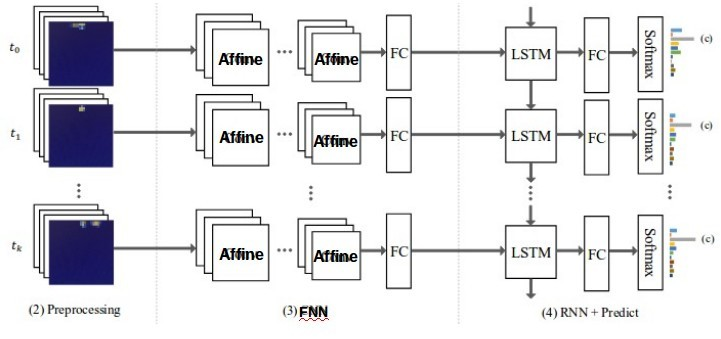
\includegraphics[width=0.99\linewidth]{./network.jpg}
\end{center}
   \caption{The FNN+RNN network architecture}
\label{fig:network}
\end{figure}

The network architecture adopted is shown in Fig \ref{fig:network}. We first chunk the time-series sensor data so that each part contains a single word. We then calculate the 17 statistical features mentioned in Table \ref{statistical_features} over the data taken in time space as well as the frequency space. We use the Fast Fourier Transform of the scikit-learn package \cite{scikit-learn} to convert the signal to frequency space. Once this is calculated, we input this array for each individual word to a 7-layer deep fully connected neural network.

The motivation behind this is for the network to learn the features it wants automatically from the hand-crafted features provided to it. We cannot provide the time-series data directly here because the sensor data has different lengths for different words, and thus initial transformation is required. These form the input data to our network. The input labels are captured by using keylogger as the ground truth and then padding the words with null characters to make them of uniform length. 

The output of the affine neural network is then input to the recurrent neural network for prediction. Since we want the affine network to learn suitable features, the network is trained end to end. This is done by implementing a fully connected layer at the end of the affine NN which outputs features for the RNN. In essence, the scores are calculated for the affine network assuming the number of classes equals the input hidden dimension to the recurrent network.

The output scores for the fully connected neural network are calculated the normal way. The initial hidden layer to the RNN then becomes:\\
$initial\_h_0=scores.dot(W_{proj})+b_{proj}$\\
The rest of the network for the RNN remains unaltered. While backpropagating the loss, we find the temporal\_softmax\_loss for the RNN and backpropagate it to get $dh_0$. For the affine network, the 'dout' of the gradient of the loss with respect to the scores is the following:\\
$dout= dh_0.dot(W_{proj}.T)$\\
Here, the different terminologies of weights and biases are the same as used in the various course assignments. The above connections help in training the affine network to output the input features desired by the RNN for successful classficiation and thus train the network end-to-end.

\begin{table}[t]
  \small
  \caption{Statistical Features}
  \label{statistical_features}
  \centering
  \begin{tabular}{|l|}
    \hline
    1. Mean: $\mu_s = \frac{1}{T} \Sigma_{i=1}^{T} s_i$ \\
    2. Standard Deviation: $\sigma_s=\sqrt{\frac{1}{T}\Sigma_{i=1}^{T}(s_i-\mu_s)}$ \\ 
    3. Coefficients of variation: $c_v=\frac{\sigma_s}{\mu_s}$ \\
    4. Peak-to-peak amplitude: $max\{s1, ..., sT\}$ - $min\{s1, .., sT\}$. \\
    5-9. Percentiles: $10^{th}$, $25^{th}$, $50^{th}$, $75^{th}$, $90^{th}$ \\
    10. Interquartile range: difference between the $75^{th}$ and $25^{th}$ \\
          \hspace{0.5cm}  percentiles. \\ 
    11. Lag-one-autocorrelation: $\frac{\Sigma_{i=1}^{T-1}(s_i-\mu_s)(s_{i+1}-\mu_s)}
    {\Sigma_{i=1}^{T}(s_{i}-\mu_s)^2}$ \\
    12. Skewness: $\frac{\frac{1}{T}\Sigma_{i=1}^{T}(s_i-\mu_s)^3}
    {(\frac{1}{T}\Sigma_{i=1}^{T}(s_i-\mu_s)^2)^{3/2}}$, measure of \\
         \hspace{0.5cm} asymmetry of the signal probability distribution. \\
    13. Kurtosis: $\frac{\frac{1}{T}\Sigma_{i=1}^{T}(s_i-\mu_s)^4}
    {(\frac{1}{T}\Sigma_{i=1}^{T}(s_i-\mu_s)^2)^{3}}-3$, degree of the \\
        \hspace{0.5cm} peakedness of the signal probability distribution. \\
    14. Signal power: $\Sigma_{i=1}^{T}s_i^2$ \\
    15. Log-energy: $\Sigma_{i=1}^{T}\log{s_i^2}$ \\
    16. Zero crossings: number of times the signal \\
         crosses its median.\\
    17. Correlation between each pair of axes: \\
     \hspace{0.5cm}$\frac{\Sigma_{i=1}^{T}(s_i-\mu_s)(v_i-\mu_v)}{\sqrt{\Sigma_{i=1}^{T}(s_i-\mu_s)\Sigma_{j=1}^{T}(v_i-\mu_v)}}$ \\
    \hline
  \end{tabular}
\end{table}


\section{Experiment}

\subsection{Data Set}
Datasets of users typing on a keyboard with smartwatches worn on both wrists aren't available on the internet. Hence, for this project, I am responsible for collecting my own data. Since we attempt to build a personalized typing predictor, we are not concerned with the lack of varied data coming from different users. To this extent, taking data from a single user (self) is deemed substantial for the project. I have collected data after having worn an ASUS ZenWatch 2 on my left wrist and a LG G Watch W100 on my right wrist. I used a self-modified version of the publicly available app Sensor Data Logger \cite{app} to record data from these smartwatches on two smartphones. The app collects data of different sensors at a preset frequency for each sensor and writes it to a file on the smartphone. This was modified and data is collected at 50 Hz for accelerometer, gyroscope and gravity sensors for this project. Gravity sensors are used to boost predictive performance, mainly because when a key is typed, there is motion in the Z axis, which can easily be picked up by gravity sensors. The app \cite{app} captures the timestamp, accurate to milliseconds, and the readings of the nine sensor axes, 3 for each sensor type.

For ground truth, I have used the publicly available Key Frequency Logger project \cite{keyfreq}, which records each typed in keystroke on the keyboard. This is accompanied by a UNIX timestamp, and the logs are stored in files for each session.

Following data collection, it is pre-processed to consider only the character set we want for our project. We have considered the 26 English alphabet letters, irrespective of case, and three special characters: '$<LShift>$','$<BkSpc>$' and '$Spc$'. The relevant characters are read from the KeyLogger file and correspondingly only the sensor data around these characters are considered for the 18 axes (9 for each hand). In the first part, we use '$Spc$' as a normal character while we are trying to classify each individual keystroke separately. However for the main FNN+RNN architecture, we use '$Spc$' to separate the words as each input example and only in essence consider (26+2) characters in the word.

For our character set in Approach 2, the size of the dataset comes out to be 15515 characters. After more processing to separate into words, and to consider only those words for which reliable sensor data is available, we are left with 1462 words. We do a 80-20 split of training and validation set on this. The validation set effectively works as the test set in this approach because we are working with RNNs. Although around 1500 examples are not substantial to train a deep network as ours, it is sufficient to show a proof of concept.

We visualize the data collected from the smartwatches. As an example, the accelerometer data from the left hand over multiple sessions of recording data is shown in Fig \ref{fig:accel_data}. We see that even though it's the same sensor for the same hand in the same position, the sensor initialization can differ a lot from session to session. Thus, it is beneficial to consider the data in frequency space than relying on their initialized accuracy.

\begin{figure}[t]
\begin{center}
   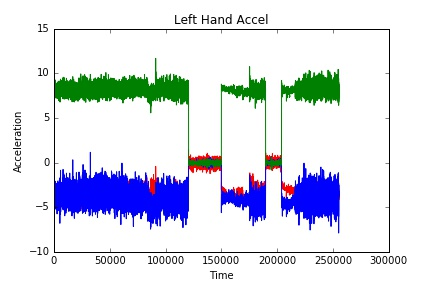
\includegraphics[width=0.99\linewidth]{./accel_data.jpg}
\end{center}
   \caption{Accelerometer data over multiple sessions from one hand}
\label{fig:accel_data}
\end{figure}

\subsection{Analysis and Results}
For the first attempt at the project, we collected data in sessions, and then transformed the data as follows. The time series data collected from the smartwatches were first aligned. This involved putting all the 18 axes of the sensors in parallel, so that we have 18 columns in the data. Signal processing tools such as the 'interpolate' function from 'scipy' \cite{scipy} were used to extrapolate the signals so that all the 18 columns have the same sample rate, something not inherent to SensorDataLogger \cite{app}.
Once this was done, we run a sliding window over the signal and compute the statistical features in the real time space as well as the Fourier space by taking the FFT transforms. This is done for each column (sensor axis) and thus, gives us a ($17*18=$)306 dimensional vector with timestamps as another column. We compress this data to have only 20 (configurable) columns using PCA, retaining the timestamp column separately. We use the timestams of individual keystrokes from the KeyFreq \cite{keyfreq} app for synchronization. We consider a window of 0.4 seconds around each keystroke and pass this as an input image to our fully connected network. The feature space before chunking the data for each keystroke is shown in Fig \ref{fig:feature_space} (a). Here, the individual keystrokes show up as blips, and we chunk the data around these blips.

The fully connected network then receives this input image (unfolded into a vector) and then attempts to classify into one of the 28 character classes. We used different network architectures, ranging from 256 to 1024 hidden nodes and 4-8 hidden layers. When considering a small number of samples (100-200), it is easy to overfit the data. However, for around 10000 characters the maximum accuracy achieved is around 26\%. Batch Normalization and Dropout are used in each of my architectures. Even though a random classifier would perform at less than 3.5\%, we realize we can do better and thus adopt the RNN approach. The confusion matrix of the overfit model for this initial approach for 100 samples is shown in Fig \ref{fig:overfit}.
\begin{figure}[t]
\begin{center}
   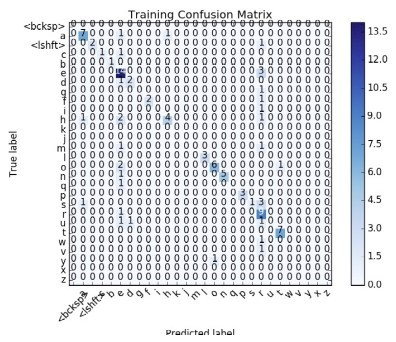
\includegraphics[width=0.99\linewidth]{./overfit_model.jpg}
\end{center}
   \caption{Overfit FNN on 100 characters}
\label{fig:overfit}
\end{figure}

The complete table of experimented values and their accuracies for 7228 characters are given in Table \ref{initial_accuracies}. A weight scale of 1e-2 is fixed since we are using batch normalization and the learning rate is cross-validated.

\begin{table}[t]
  \small
  \caption{Performance of Fully Connected Network in Approach 1}
  \label{initial_accuracies}
  \centering
  \begin{tabular}{l|l|l|l|l}
    \hline
    \#Hidden Layers & PCA Comp & Dropout & Reg & Accuracy \\
    \hline
    4 & 20 & 0.1 & 1e-6 & 13.14\\
    7 & 20 & 0.1 & 1e-6 & 15.17\\
    7 & 20 & 0.25 & 1e-6 & 14.82\\
    7 & 30 & 0.1 & 1e-5 & 17.59\\
    11 & 30 & 0.1 & 1e-6 & $\mathbf{25.93}$\\
    11 & 30 & 0.25 & 1e-5 & 22.74\\
    \hline
  \end{tabular}
\end{table}

For the RNN approach, we use a slightly different feature space. We begin by clustering the characters into a word depending on the '$Spc$' character. Then we take the sensor data around the whole word with a padding of 0.4 seconds around each word. Once we have this time series data for a word, we realize they are of different lengths for different words and extrapolating them is not beneficial. Hence, we calculate the 17 statistical features over every sensor type in the real time space as well as the frequency space, normalize it across its 3 axes, and then horizontally stack the calculated features. Since we have 6 sensor types (3 for each type), and we consider real as well as Fourier space, we get an input image matrix of 204 ($6*2*17$) rows and 3 columns (each axis of sensor type). An example input image is shown in Fig \ref{fig:feature_space} (b).

\begin{figure}[t]
\begin{center}
   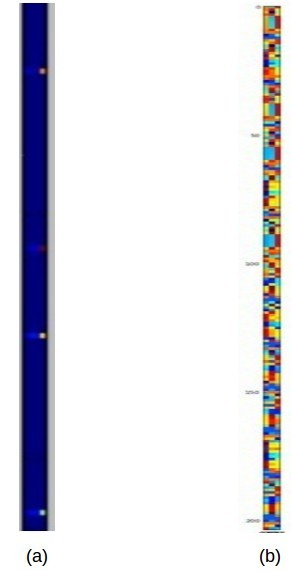
\includegraphics[width=0.4\linewidth]{./feature.jpg}
\end{center}
   \caption{Input Feature Space for the two approaches}
\label{fig:feature_space}
\end{figure}

This image is then expanded into a one-dimensional vector, compressed to 300 dimensions using PCA (from 612 dimensional) and input into a fully connected neural network for appropriate feature extraction. The affine network consists of 7 fully connected layers, each layer with 512 nodes. The code from assignment 2 of the course is extensively used for our network implementation.

We then pass the output of the affine NN as the initial features to the RNN. On the lines of assignment 3, we consider each individual character as a character vector. The words consist of a '$<START>$' token, a '$<END>$' token and '$<NULL>$' tokens as the padding to make the word length uniformly equal to 17 characters for all samples. The input features to RNN are then used as the initial hidden layer and the '$<START>$' token as the initial input data. It is then trained to predict the other characters.

Training a model this way has the added feature that it learns the context of a letter against the backdrop of other letters. Hence, it is not restricted to English words, although they could be used to boost performance by pattern matching. Hence, the model can learn each individual person's typing behaviour pattern.

The results of the RNN are evaluated aesthetically instead of calculating the accuracy over the entire predictions. This is done because a sample will be classified as wrongly predicted even if the RNN wrongly predicts only the last letter. We are instead interested in the general performance of the RNN to show as proof of concept. The evaluation metric for choosing the best hyperparameter values for the affine and the recurrent network is instead the raw loss value which is returned by '$temporal\_softmax\_loss$' method of RNN, regularized with the sum of the L2 norm of the weights of the fully connected network.

A few of these predictions along with their ground truth are shown in Table \ref{rnn_predictions}. As we can see, even for the validation set, the predicted words are not very different from the ground truth. Furthermore, we see that even though the results are not identical, they are similar for the most part. Also, we see that the features passed on to the RNN from FNN definitely has information regarding the length of a word because the predicted words have approximately the same length as the ground truth, even if the characters themselves do not entirely match.

\begin{table}[t]
  \small
  \caption{Network Predictions in Approach 2}
  \label{rnn_predictions}
  \centering
  \begin{tabular}{l|l|l}
    \hline
    Split & Ground Truth & Sampled \\
    \hline
    Train & \verb'<START>the<END>' & \verb'the<END>'\\
    Train & \verb'<START>five<END>' & \verb'five<END>'\\
    Train & \verb'<START>where<END>' & \verb'poor<END>'\\
    Validation & \verb'<START>house<END>' & \verb'bore<END>'\\
    Validation & \verb'<START>purpose<END>' & \verb'poonere<END>'\\
    \hline
  \end{tabular}
\end{table}

\section{Conclusion}
The results show that the the network can predict the typed words to a fair degree of similarity. Since it is difficult to measure accuracy directly, we notice that the essence of the word is retained. Since the model is only trained over around 1000 samples (words), the network doesn't get enough time to learn the context over characters exactly. However, in most cases, we see that it still manages to predict an English dictionary word, since all of our training samples were actual English words.

The fact that Approach 2 in general performs better than Approach 1 shows that letting a network learn the feature space on its own pays off. The end-to-end network was able to inherit information like the length of the words, whereas any hand-made features would not have performed equally. Further, the network shows that characters are a lot more prone to appear in the context of other characters in the English language. We didn't provide the network with any dictionary of the English language and yet, even the wrongly predicted words were legitimate. This shows that a lot more relevant information goes in the feature space developed by the FNN which boosts the predictive power of RNN.

Given more time, the key things to try out would be firstly to get a much larger data set of a lot more words and see if the model improves its performance. This is intuitive but the extent of the scalability would be interesting. Second, I would like to try out more (or fewer) sensors, to see if the predictive performance goes up. To be able to get maximum performance with the minimum sensors would be the goal, since recording data over various sensors depletes the battery of the smartwatch at a faster pace. Third, I would experiment whether the model can predict the intended word being typed if I recorded data of my hand typing (based off only muscle memory) on a flat platform like a wooden desk.

A key area of further investigation could be crafting of new features. We provide the affine network with the statistical features which have traditionally been robust. Even though we provide it in both frequency and time space, it would be interesting to see the results if we extrapolated the signals for each word to the same length and passed this signal itself to the FNN. We have seen that the FNN is capable of extracting strong features, and thus should be able to make the best use of the raw signal. Despite this, our project shows that the end-to-end model learns the characters and their contexts fast given the number of training samples.

\begin{thebibliography}{1}
  \small
  \bibitem{bonomi}  Bonomi, A. G., Goris, A. H. C., Yin, B.\ \& Westerterp, K. R. (2009) Detection of Type, Duration, and Intensity of Physical Activity Using an Accelerometer. {\it Medicine \& Science in Sports \& Exercise}, 2009 Sep, pp.\ 1770--1777.
  \bibitem{weiss} Kwapisz, J. R., Weiss, G. M.\ \& Moore, S. A. (2010) Activity Recognition using Cell Phone Accelerometers. {\it ACM SIGKDD Explorations Newsletter}, 2010 Dec, pp.\ 74--82.
  \bibitem{mannini} Mannini, A., Intille, S.S., Rosenberger, M., Sabatini, A. M., and Haskell, W. (2013) Activity recognition using a single accelerometer placed at the wrist or ankle. {\it Medicine \& Science in Sports \& Exercise}, 2013 Nov, pp.\ 2193--2203.
  \bibitem{zheng} Zheng, Y., Wong, W., Guan, X.\ \& Trost, S. (2013) Physical Activity Recognition from Accelerometer Data Using a Multi-Scale Ensemble Method. {\it Innovative Applications of Artificial Intelligence}, pp. 1575--1581.
  \bibitem{ravi} Ravi, N., Dandekar, N., Mysore, P.\ \& Littman, M. L (2005) Activity Recognition from Accelerometer Data. {\it Innovative Applications of Artificial Intelligence}, pp.\ 1541--1546.
  \bibitem{wang} He Wang, Ted Tsung-Te Lai, \& Romit Roy Choudhury (2015) MoLe: Motion Leaks through Smartwatch Sensors. {\it MobiCom 2015}
  \bibitem{maiti} Anindya Maiti, Oscar Armbruster, Murtuza Jadliwala, \& and Jibo He (2016) Smartwatch-Based Keystroke Inference Attacks and
Context-Aware Protection Mechanisms. {\it ASIA CCS 2016}
  \bibitem{dunn} Li X, Dunn J, Salins D, Zhou G, Zhou W, Schüssler-Fiorenza Rose SM, et al. (2017) Digital Health: Tracking Physiomes and Activity Using Wearable Biosensors Reveals Useful Health-Related Information. {\it PLoS Biol15(1)}
  \bibitem{scipy} Jones E, Oliphant E, Peterson P, et al. SciPy: Open Source Scientific Tools for Python, 2001-, http://www.scipy.org/ [Online; accessed 2017-12-20]
  \bibitem{scikit-learn} Pedregosa, F., Varoquaux, G., Gramfort, A., Michel, V., Thirion, B., Grisel, O., Blondel, M., Prettenhofer, P., Weiss, R., Dubourg, V., Vanderplas, J., Passos, A., Cournapeau, D., Brucher, M., Perrot, M.\ \& Duchesnay, E. (2011) Scikit-learn: Machine Learning in Python. {\it Journal of Machine Learning Research}, 12, pp. 2825--2830
  \bibitem{messenger} {\it Facebook Messenger} - Available on Play Store for direct installation by Facebook. Also available at \url{https://www.facebook.com/messenger}
  \bibitem{app} {\it Sensor Data Logger} - open-source Android Wear app, available on GitHub at \url{https://github.com/Steppschuh/Sensor-Data-Logger}. Also available on Play Store for direct installation.
  \bibitem{keyfreq} {\it Key Frequency Logger} - open-source Git Project, available at \url{https://github.com/bagder/keyfreq}
\end{thebibliography}

\end{document}
